Il suffit effectivement de concevoir un ressort appliqu\'{e} seulement \`{a} l'un des
\edtext{obstacles $\displaystyle CD$, ou}{\lemma{obstacles $\displaystyle CD$,}\Bfootnote{ \textit{ (1) }\ et \textit{ (2) }\ ou \textit{ L}}}
$\displaystyle EF$.
\pend
\vspace{1.5em}
\pstart
\centering
\noindent
    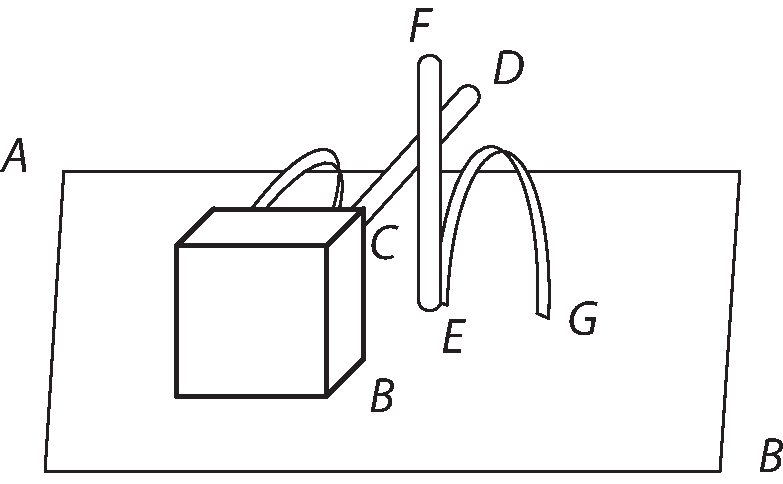
\includegraphics[width=0.48\textwidth]{images/lh0350911_008v_2-d1.pdf}\pend
    \vspace{2mm}
    \pstart
    \centering
    [\textit{Fig. 1}]% \caption{Bildbeschreibung}
    \pend
    \newpage
\pstart
\centering
[\textit{Teil 2}]
%\vspace{0,5em}
\pend
\count\Bfootins=1000
\count\Cfootins=1000
\count\Afootins=1000
\pstart
\noindent
Si ponamus decrementa esse uniformia, quae a frictione\protect\index{Sachverzeichnis}{frictio} uniformi oriuntur,
erunt celeritates\protect\index{Sachverzeichnis}{celeritas} ut applicatae Trianguli,
sive erunt celeritates $\displaystyle BC$ ut spatia $\displaystyle AB$, sumta a puncto
cessationis, seu ut spatia percurrenda\protect\index{Sachverzeichnis}{spatium percurrendum} residua, sunt autem momenta temporum
quibus spatia minora quam quae assignari possint percurruntur, ipsis celeritatibus reciproce proportionalia;
sunt ergo temporum incrementa ut applicatae
\edtext{hyperbolae $\displaystyle BD.$}{\lemma{hyperbolae}\Bfootnote{\textit{(1)}\ : ergo \textit{(2)}\ $\displaystyle BD.$ \textit{L}}}
tempora \edtext{ipsa ut quadrilinea Hyperbolica}{\lemma{ipsa}\Bfootnote{\textit{(1)}\ ut Logarithmi \textit{(2)}\ ut  \textit{(a)}\ Logari \textit{(b)}\ spatia \textit{(c)}\ portiones Hyperbolicae \textit{(d)}\ quadrilinea Hyperbolica \textit{L}}}
$\displaystyle FEBDF$. Ergo si
\edtext{spatia percurrenda $\displaystyle AB.$ $\displaystyle A(B).$ $\displaystyle A((B))$ sint ut numeri,
erunt tempora insumenda donec ad terminum perveniatur,
ut spatia [$\displaystyle HABDGH$] seu ut rectae $\displaystyle AL$, $\displaystyle BN$.}{\lemma{spatia}\Bfootnote{%
\textit{(1)}\ \textbar\ percursa \textit{erg.}\ \textbar\ $\displaystyle EB$, $\displaystyle E(B)$, $\displaystyle E((B))$ sint ut numeri, tempora insumta erunt ut Logarithmi %
\textit{(2)}\ percurrenda $\displaystyle AB.$ %
\textit{(a)}\ sint %
\textit{(b)}\ $\displaystyle A(B).$ $\displaystyle A((B))$ sint [...] tempora %
\textit{(aa)}\ insumta %
\textit{(bb)}\ insumenda %
\textit{(aaa)}\ motu %
\textit{(bbb)}\ donec [...] spatia %
\textit{(aaaa)}\ $\displaystyle GABGHG$ %
\textit{(bbbb)}\ $\displaystyle GABHG$ seu ut rectae $\displaystyle AL$, $\displaystyle BN$. \textit{L ändert Hrsg.}}}%
\edtext{}{\lemma{ut rectae $\displaystyle AL$, $\displaystyle BN$}\Cfootnote{%
Bei den sechs eingeklammerten Gro{\ss}buchstaben in der Zeichnung [\textit{Fig. 2}] sind die Klammern vom Hrsg. erg\"{a}nzt. Die Punkte, die im Text durch doppelt eingeklammerte Gro{\ss}buch\-staben bezeichnet werden, sind in der Zeichnung nicht abgebildet. Ferner werden in [\textit{Fig. 2}] mit dem gleichen Gro{\ss}buchstaben $\displaystyle H$ verschiedene Punkte bezeichnet.}}
\pend
\pstart 
Recte et rigorose concipienda res \edtext{est:\\
\hspace*{7,5mm}Hyperbolae centrum $\displaystyle A$. Asymptoti}{\lemma{est:}\Bfootnote{\textit{(1)}\ Asymptoti \textit{(2)}\ Hyperbolae  \textit{(a)}\ vertex $\displaystyle A$ \textit{(b)}\ centrum $\displaystyle A$. Asymptoti \textit{L}}}
sunt $\displaystyle AH$, $\displaystyle AE$.
In asymptoto $\displaystyle AE$, terminata ubilibet in $\displaystyle E$,
sumatur inter $\displaystyle A$ et $\displaystyle E$ punctum aliquod $\displaystyle P$
et ducatur $\displaystyle PQ$ ad Hyperbolam applicata.
Per demonstrata a Gregorio a
\edtext{S. Vincentio\protect\index{Namensregister}{\textso{Saint-Vincent}, Gr\'{e}goire de (Gregorius a S. Vincentio) S.J. 1584-1667}}{\lemma{S. Vincentio}\Cfootnote{\cite{00316}G. \textsc{de Saint Vincent}, \textit{Opus geometricum}, Antwerpen 1647, lib. VI, prop. 129, S. 596f.}}
(:~quae repetit \edtext{Wallis\protect\index{Namensregister}{\textso{Wallis} (Wallisius), John 1616-1703}\edtext{}{\lemma{}\Afootnote{\textit{Am Rand:} Debuisset dicere Wallisius\protect\index{Namensregister}{\textso{Walli}s (Wallisius), John 1616-1703}. $\displaystyle AB.$ $\displaystyle A(B).$ $\displaystyle AE.$ Vid. Mercator\protect\index{Namensregister}{\textso{Mercator}, Nicolaus 1620-1687}\textsuperscript{[a]}.\vspace{2mm}\\% PR: Marginalienapparat:
\footnotesize
\textsuperscript{[a]} Mercator:\ \ %N. \textsc{Mercator},
\textsc{N. Mercator}, \cite{00141}\textit{Logarithmotechnia}, London 1668, prop. XIVf., S.~28f. Leibniz hat in seinem Ex\-em\-plar der \textit{Logarithmotechnia} beide Theoreme kommentiert: Siehe \cite{01189}\textit{LSB} VII,~4 N.~3\textsubscript{1}, S.~50f.\vspace{-8mm}}}
in \textit{transact.} 38}{\lemma{Wallis in \textit{transact.} 38}\Cfootnote{\cite{00236}J. \textsc{Wallis}, \textit{Logarithmotechnia Nicolai Mercatoris}, in \textit{PT} III, Nr. 38, 17. (27.) August 1668, S. 753-759.}}~:)
si $\displaystyle PB.$ $\displaystyle P(B)$
\edtext{etc.}{\lemma{}\Bfootnote{etc. \textit{erg. L}}}
usque ad $\displaystyle PE$
\edtext{vel etiam porro si placet}{\lemma{}\Bfootnote{vel [...] placet \textit{erg. L}}}
sint ut numeri, erunt spatia $\displaystyle QPBDQ$, $\displaystyle QP(B)(D)Q$ etc. usque ad $\displaystyle QPEFQ$
\edtext{vel etiam porro si placet}{\lemma{}\Bfootnote{vel [...] placet \textit{erg.} \textit{L}}}
ut Logarithmi.
Ergo si $\displaystyle P$ colloces in ipso centro $\displaystyle A$
eodem modo dicemus, si finitae $\displaystyle AB$, $\displaystyle A(B)$
\edtext{etc.}{\lemma{}\Bfootnote{etc. \textit{erg. L}}}
usque ad $\displaystyle AE$, vel etiam porro si placet sunt ut numeri, erunt spatia
\edtext{infinita $\displaystyle HABDGH.$ $\displaystyle HA(B)(D)GH$ etc.}{\lemma{infinita}\Bfootnote{\textit{(1)}\ $\displaystyle HA(B)QGH.$ \textit{(2)}\  $\displaystyle HABDGH.$ $\displaystyle HA(B)(D)GH$ etc. \textit{ L}}}
\edtext{usque ad $\displaystyle HAEFGH$ vel etiam porro si placet, ut}{\lemma{usque ad}\Bfootnote{%
\textit{(1)}\ $\displaystyle HAEDGH$ %
\textit{(2)}\ $\displaystyle HAEFGH$ %
\textit{(a)}\ ut %
\textit{(b)}\ vel [...] ut \textit{L}}}
Logarithmi.
\pend
\newpage
\pstart 
\noindent
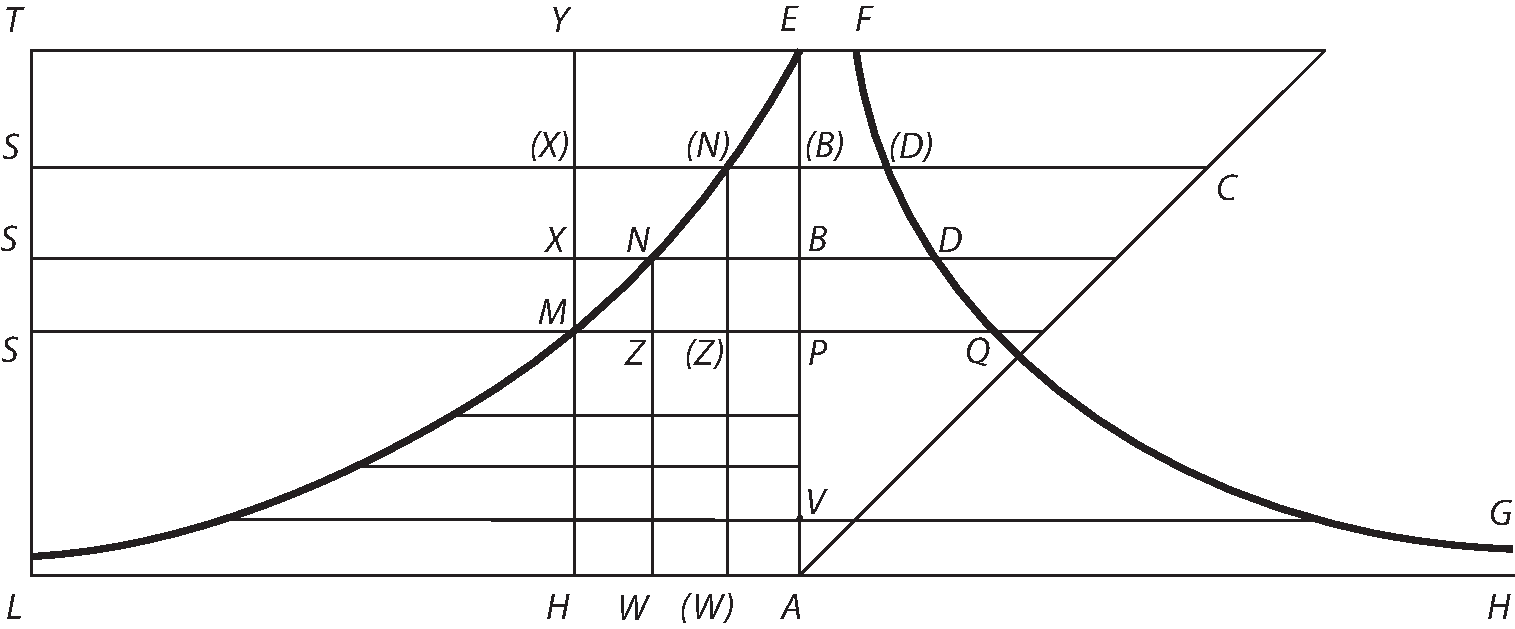
\includegraphics[trim = 0mm -3mm 0mm 0mm, clip, width=0.99\textwidth]{images/lh0350911_009r-d1.pdf}
    \centering
    [\textit{Fig. 2}] % \caption{Bildbeschreibung}
\pend
\count\Bfootins=1200
\count\Cfootins=1200
\count\Afootins=1200
\vspace{6mm}
\pstart
Quod si \setline{1}jam lineam
\edtext{describamus $\displaystyle ENM$}{\lemma{describamus}\Bfootnote{\textit{(1)}\ $\displaystyle RNM.$ \textit{(2)}\ $\displaystyle ENM$ \textit{L}}}
quae etiam duas habet Asymptotos $\displaystyle AL$, et $\displaystyle AE$
ita ut applicatae
\edtext{ejus $\displaystyle BN.$ $\displaystyle (B)(N)$}{\lemma{ejus}\Bfootnote{\textit{(1)}\ $\displaystyle RE.$, \textit{(2)}\  $\displaystyle BN.$ $\displaystyle (B)(N)$ \textit{L}}}
usque ad infinitum $\displaystyle AL$
sint spatiis $\displaystyle FEBDF.$ $\displaystyle FE(B)(D)F$ etc.
usque ad spatium infinitum $\displaystyle FEAHGF$ proportionales,
et intelligantur rectae $\displaystyle BN.$ $\displaystyle (B)(N)$ in infinitum productae,
ita ut aequentur Asymptoto, $\displaystyle AL$,
ac proinde ut puncta $\displaystyle S.$ $\displaystyle (S)$ a punctis $\displaystyle B.$ $\displaystyle (B)$ tanto distent intervallo infinito,
quanto punctum $\displaystyle L$ a puncto $\displaystyle A$[,]
erunt 
\edtext{rectae infinitae $\displaystyle TE.$ $\displaystyle (S)(N).$ $\displaystyle SN$ ut spatia infinita, $\displaystyle HAEFGH.$ $\displaystyle HA(B)(D)GH.$ $\displaystyle HABDGH$ seu ut logarithmi numerorum finitorum $\displaystyle AE.$ $\displaystyle A(B).$ $\displaystyle AB.$}{\lemma{rectae}\Bfootnote{\textit{(1)}\ $\displaystyle LA$ \textit{(2)}\ infinitae  \textit{(a)}\ $\displaystyle SA$ $\displaystyle LA$,  \textit{(aa)}\ $\displaystyle SN$ \textit{(bb)}\ $\displaystyle A(B)$ \textit{(b)}\ $\displaystyle TE.$ $\displaystyle SN.$ $\displaystyle (S)(N).$  \textit{(aa)}\ $\displaystyle AL.$ \textit{(bb)}\ ut spatia infinita $\displaystyle HAEFGH.$ \textit{(c)}\ $\displaystyle TE.$  \textit{(aa)}\ $\displaystyle (S)(N)$ \textit{(bb)}\ $\displaystyle (S)(N).$ $\displaystyle SN$ ut [...]  $\displaystyle AE.$ $\displaystyle A(B).$ $\displaystyle AB.$ \textit{L}}}
%\edtext{rectae infinitae $\displaystyle TE.$ $\displaystyle (S)(N).$ $\displaystyle SN$ ut spatia infinita, $\displaystyle HAEFGH.$ $\displaystyle HA(B)(D)GH.$ $\displaystyle HABDGH$ seu ut logarithmi numerorum finitorum $\displaystyle AE.$ $\displaystyle A(B).$ $\displaystyle AB$}{\lemma{rectae}\Bfootnote{\textit{(1)}\ $\displaystyle LA$ \textit{(2)}\ infinitae  \textit{(a)}\ $\displaystyle SA$ $\displaystyle LA$,  \textit{(aa)}\ $\displaystyle SN$ \textit{(bb)}\ $\displaystyle [...] A(B)$ \textit{(b)}\ $\displaystyle TE.$ $\displaystyle SN.$ $\displaystyle (S)(N).$  \textit{(aa)}\ $\displaystyle AL.$ \textit{(bb)}\ ut spatia infinita $\displaystyle HAEFGH.$ \textit{(c)}\ $\displaystyle TE.$ $\displaystyle (S)(N).$  \textit{(aa)}\ $\displaystyle (S)(N)$ \textit{(bb)}\ $\displaystyle (S)(N).$ $\displaystyle SN$ ut [...]  $\displaystyle AE.$ $\displaystyle A(B).$ $\displaystyle AB$ \textit{L}}}.
Unde apparet corollarium mirabile, logarithmos numerorum
\edtext{finitorum infinitis}{\lemma{finitorum}\Bfootnote{\textit{(1)}\ infinitos \textit{(2)}\ infinitis \textit{L}}}
modis assumi posse, et aliquando ita,
ut logarithmi eorum repraesententur quantitatibus infinitis finito intervallo
\edtext{differentibus, id est}{\lemma{differentibus,}\Bfootnote{\textit{(1)}\ ut \textit{(2)}\ id est \textit{L}}}
aequalibus quia et termini aequales progressionis geometricae sunt.
Unde patet non nisi infinito tempore mobile pervenire posse ad terminum $\displaystyle A$
atque ideo non punctum $\displaystyle A$ calculi causa pro termino motus sumendum,
sed \edtext{aliquod quodcunque quantulocunque intervallo citerius}{\lemma{aliquod}\Bfootnote{\textit{(1)}\ citerius \textit{(2)}\ quodcunque [...] citerius, \textit{L}}},
ut $\displaystyle P$, ita ut $\displaystyle PM$ sit finita, et tunc ex puncto $\displaystyle M$ 
[erigendam]\edtext{}{\lemma{erigendo}\Bfootnote{\textit{\ L \"{a}ndert Hrsg.}}}
parallelam ipsi $\displaystyle AE$.
% [9~v\textsuperscript{o}]
% \pend